\documentclass[12pt]{article}
\usepackage[utf8]{inputenc}
\usepackage[dvips]{graphicx}
\usepackage{epsfig}
\usepackage{fancybox}
\usepackage{verbatim}
\usepackage{array}
\usepackage{latexsym}
\usepackage{alltt}
\usepackage{amssymb}
\usepackage{amsmath}
\usepackage{hyperref}
\usepackage{listings}
\usepackage{color}
\usepackage{algorithm}
\usepackage{algpseudocode}
\usepackage[hmargin=3cm,vmargin=5.0cm]{geometry}
\usepackage{epstopdf}
\graphicspath{ {./images/} }
\usepackage{caption}
\usepackage{tikz}
\usepackage{pgfplots}
\usepackage{multirow}
\usepackage{hyperref}
\hypersetup{
    colorlinks=true,
    linkcolor=blue,
    filecolor=magenta,      
    urlcolor=cyan,
}
\urlstyle{same}
\topmargin=-1.8cm
\addtolength{\textheight}{6.5cm}
\addtolength{\textwidth}{2.0cm}
\setlength{\oddsidemargin}{0.0cm}
\setlength{\evensidemargin}{0.0cm}
\newcommand{\HRule}{\rule{\linewidth}{1mm}}
\newcommand{\kutu}[2]{\framebox[#1mm]{\rule[-2mm]{0mm}{#2mm}}}
\newcommand{\gap}{ \\[1mm] }
\newcommand{\Q}{\raisebox{1.7pt}{$\scriptstyle\bigcirc$}}
\newcommand{\minus}{\scalebox{0.35}[1.0]{$-$}}



\lstset{
    %backgroundcolor=\color{lbcolor},
    tabsize=2,
    language=MATLAB,
    basicstyle=\footnotesize,
    numberstyle=\footnotesize,
    aboveskip={0.0\baselineskip},
    belowskip={0.0\baselineskip},
    columns=fixed,
    showstringspaces=false,
    breaklines=true,
    prebreak=\raisebox{0ex}[0ex][0ex]{\ensuremath{\hookleftarrow}},
    %frame=single,
    showtabs=false,
    showspaces=false,
    showstringspaces=false,
    identifierstyle=\ttfamily,
    keywordstyle=\color[rgb]{0,0,1},
    commentstyle=\color[rgb]{0.133,0.545,0.133},
    stringstyle=\color[rgb]{0.627,0.126,0.941},
}


\begin{document}

\noindent
\HRule %\\[3mm]
\small
\begin{center}
	\LARGE \textbf{CENG 483} \\[4mm]
	\Large Introduction to Computer Vision \\[4mm]
	\normalsize Spring 2018-2019 \\
	\Large Take Home Exam 2 \\
	\Large Object Recognition \\
    \Large Student Random ID: 70 \\
\end{center}
\HRule

\begin{center}
\end{center}
\vspace{-10mm}

\section{Local Features (15 pts)}

    \begin{itemize}
        \item Explain SIFT and Dense-SIFT in your own words. What is the main difference?
        
        The main difference is that generation of keypoints of an image. The keypoints are generated with step size, x and y coordinates of an image in Dense-SIFT whereas the keypoints are obtained from various steps in SIFT. Those steps are obtaining Difference of Gaussian, finding possible local features (keypoints) which are the local extremas over scale and space in DoG, and refinement process of local features. After the generation of keypoints, their descriptors are obtained. Keypoint differences can be seen below:
        
        \begin{figure}[h]
			\centering
			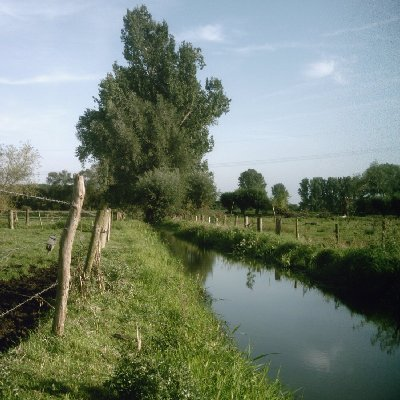
\includegraphics[width=0.32\textwidth]{example1.jpg}
			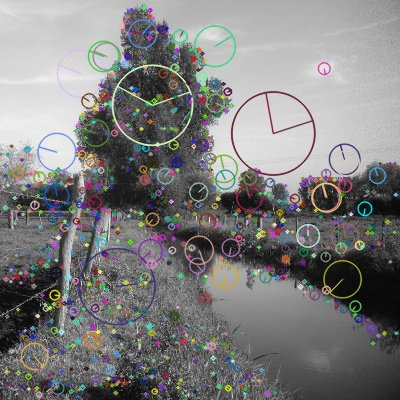
\includegraphics[width=0.32\textwidth]{example1_sift_keypoints.jpg}
			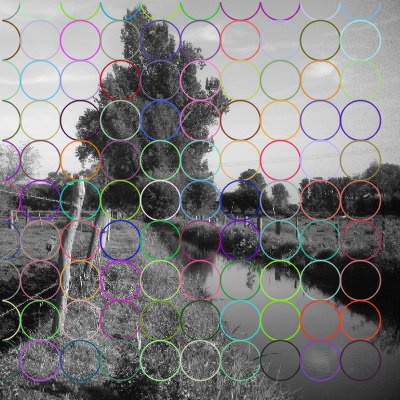
\includegraphics[width=0.32\textwidth]{example1_densesift_keypoints.jpg}
			\caption{An example image and visualizations of its keypoints from SIFT and Dense-SIFT respectively}
		\end{figure}
		
		I mentioned about various steps of obtaining local features in SIFT above, those steps form SIFT parameters such as number of features, number of octave layers, contrast threshold value, edge threshold value, sigma value. Different parameters cause differences in obtaining keypoints:
        
        \begin{figure}[h]
			\centering
			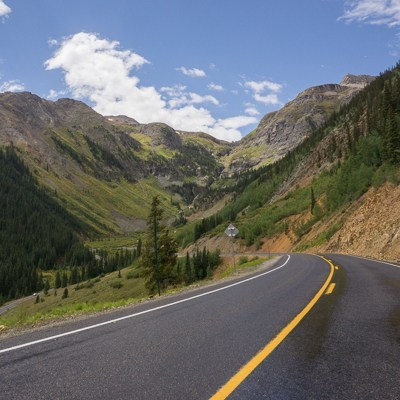
\includegraphics[width=0.32\textwidth]{example2.jpg}
			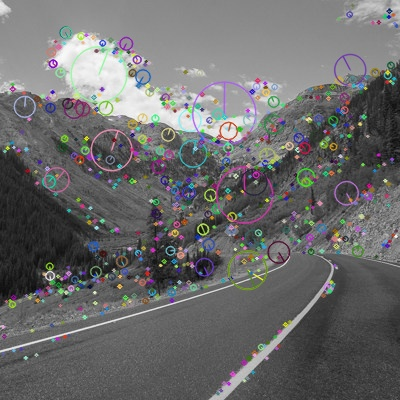
\includegraphics[width=0.32\textwidth]{example2_sift_default.jpg}
			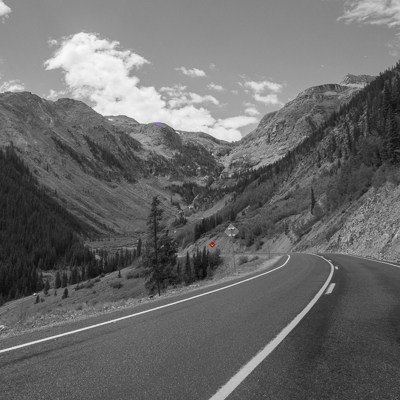
\includegraphics[width=0.32\textwidth]{example2_sift_parameter.jpg}
			\caption{An example image and visualizations of its keypoints with different SIFT parameters. The first one's parameters are default which is nfeatures=0, nOctaveLayers=3, contrastThreshold=0.04, edgeThreshold=10, sigma=1.6. The second one's parameters are nfeatures=0, nOctaveLayers=3, contrastThreshold=0.014, edgeThreshold=10, sigma=0.27.}
		\end{figure}
        \pagebreak
        \item Put your quantitative results (classification accuracy) regarding several values of SIFT and Dense-SIFT parameters here. Discuss the effect of these parameters.
        
        Using SIFT feature descriptor with given parameters resulted poorly for small values of \textbf{k}'s such as k-means 16, 32 and k-nearest neighbor 1, 2. Therefore, I compared SIFT and Dense-SIFT descriptors with k-means 64 and k-nearest neighbor 4 due to better and much more comparable accuracy results. I thought Dense-SIFT would have better accuracy with small step size values as it summarizes the whole image with its generated keypoints. However, increasing the step size would result in decreasing the accuracy. I obtained Dense-SIFT accuracies for step size 2, 3, 4, 7 and 15. Step size 0 corresponds to SIFT.
        
        \begin{minipage}{\textwidth}
			\begin{minipage}{0.49\textwidth}
				\centering
				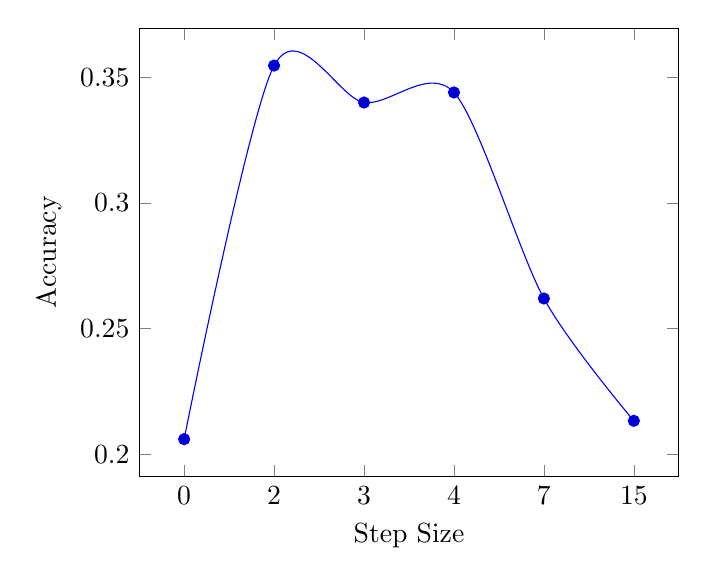
\begin{tikzpicture}
				    \begin{axis}
				        [
				        ,xlabel=Step Size
				        ,ylabel=Accuracy
				        ,yticklabel style={/pgf/number format/fixed}
				        ,xtick=data,
				        ,xticklabels={0, 2, 3, 4, 7, 15}
				        ]
				        \addplot+[smooth] coordinates
				        {(0,0.206) (1,0.3547) (2,0.34) (3,0.344) (4,0.262) (5,0.2133)};
				    \end{axis}
				\end{tikzpicture}
				\captionsetup{width=.9\textwidth}
				\captionof{figure}{Accuracy results with different step sizes where k-means and k-nearest neighbor values are 64 and 4 respectively.}
			 \end{minipage}
			 \hfill
			\begin{minipage}{0.49\textwidth}
				\centering
				\begin{tabular}{ | c | c | }
				  \hline			
				  \bf step size & \bf accuracy \\
				  \hline		
				  0 & 0.206 \\
				  \hline	
				  2 & 0.3547 \\
				  \hline	
				  3 & 0.34 \\
				  \hline	
				  4 & 0.344 \\
				  \hline	
				  7 & 0.262 \\
				  \hline	
				  15 & 0.2133 \\
				  \hline
				\end{tabular}
				\captionsetup{width=.8\textwidth}
				\captionof{table}{Accuracy results with different step sizes where k-means and k-nearest neighbor values are 64 and 4 respectively.}
			\end{minipage}
		\end{minipage} \\
		
		As it can be seen above, accuracy of SIFT descriptor is pretty lower than Dense-SIFT with small step sizes. That's probably caused by obtanining insufficient amount of keypoints from SIFT. SIFT's accuracy can be increased by tuning the SIFT parameters such as \textit{nfeatures}, \textit{nOctaveLayers}, \textit{contrastThreshold}, \textit{edgeThreshold}, \textit{sigma}. However, Dense-SIFT with smaller step sizes will get higher accuracy than SIFT in terms of classification. Higher step size in Dense-SIFT also gets lower accuracy.
    \end{itemize}


\section{Bag of Features (35 pts)}
    \begin{itemize}
        \item How did you implement BoF? Briefly explain.
        
		SIFT local feature descriptor is a vector with 128 values. I obtained local feature descriptors (with SIFT or Dense-SIFT) from each image in the train dataset and collected them together. Their collections is a matrix of size $N*128$ where $N$ is the number of obtained descriptors from the train dataset. And then, I applied KMeans algorithm to that collection in order to obtain \textit{k-cluster center}s where each center is vector of length 128. Those cluster centers are representing the dictionary. After the dictionary is formed, an image's local features are assigned to closest centers. Features' assignations to cluster centers are transformed into a normalized histogram which will be the Bag of Feature representation of an image.
        
        \item Give pseudo-code for obtaining the dictionary.
        
	        \begin{lstlisting}[language=Python]
	kmeans = 64	# 16, 32, 64 or 128
	descriptor_list = []	# List of all feature descriptors
	        	
	for image in ValidationImages:
		descriptors = extract_local_features(image)	# List of extracted feature descriptors of an image
		descriptor_list.extend(descriptors)
		
	kmeans = KMeans(n_clusters=k_means, random_state=0).fit(descriptor_list)	# or MiniBatchKMeans instead of KMeans, in order to obtain KMeans model
			\end{lstlisting}
        
        \item Give pseudo-code for obtaining BoF representation of an image once the dictionary is formed. 
        
	        \begin{lstlisting}[language=Python]
	descriptors = extract_local_features(image)	# List of extracted feature descriptors of an image
	descriptor_centers = kmeans.predict(descriptors)	# List of predicted centers of extracted feature descriptors
	histogram, _ = np.histogram(descriptor_centers, bins=range(k_means+1), normed=True)	# Bag of Feature representation of an image
			\end{lstlisting}
			
        \item Put your quantitative results (classification accuracy) regarding several values of BoF parameters here (e.g. $k$ of k-means algorithm). Discuss the effect of these.
        
        We have lots of feature descriptors from different images and we cannot be sure what the features and also the cluster centers represent. For example, we cannot say that one of the center is definitely representing a particular feature such as cat's ear, dog's nose etc. Therefore, having sufficiently many cluster centers would be better for higher accuracy as different features can be seperated from each other. However, having extremely many cluster centers decreases the accuracy because similar features might get separated from each other due to having unnecessarily many cluster centers. Thus, it's expected to see an increase of accuracy when the $k$ value of k-means algorithm increased and a decrese of accuracy when the $k$ value of k-means algorithm is large.
        
        I obtained accuracy values for k-means value 16, 32, 64 and 128 with k-nearest neigbor value 4 with different local feature descriptor.
        
        \begin{minipage}{\textwidth}
			\begin{minipage}{0.49\textwidth}
				\centering
				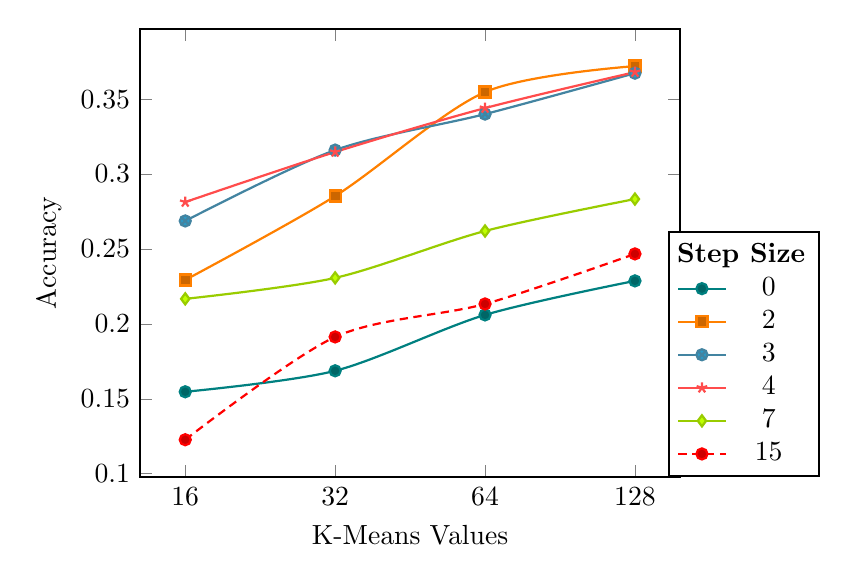
\begin{tikzpicture}
				    \begin{axis}
				        [
				        ,xlabel=K-Means Values
				        ,ylabel=Accuracy
				        ,yticklabel style={/pgf/number format/fixed}
				        ,xtick=data
				        ,xticklabels={16, 32, 64, 128}
				        ,legend style={at={(1.26 ,0.00)},anchor=south east}
				        ,cycle list name=exotic
				        ,smooth
				        ,thick
				        ,mark=*
				        ]
   						\addlegendimage{empty legend}
				        \addplot coordinates
				        {(0,0.1547) (1,0.1687) (2,0.206) (3,0.2287)};
				        \addplot coordinates
				        {(0,0.2293) (1,0.2853) (2,0.3547) (3,0.372)};
				        \addplot coordinates
				        {(0,0.2687) (1,0.316) (2,0.34) (3,0.3673)};
				        \addplot coordinates
				        {(0,0.2813) (1,0.3147) (2,0.344) (3,0.368)};
				        \addplot coordinates
				        {(0,0.2167) (1,0.2307) (2,0.262) (3,0.2833)};
				        \addplot coordinates
				        {(0,0.1227) (1,0.1913) (2,0.2133) (3,0.2467)};
				        \addlegendentry{\hspace{-.7cm}\textbf{Step Size}};
   						\addlegendentry{0}
   						\addlegendentry{2}
   						\addlegendentry{3}
   						\addlegendentry{4}
   						\addlegendentry{7}
   						\addlegendentry{15}
				    \end{axis}
				\end{tikzpicture}
				\captionsetup{width=.9\textwidth}
				\captionof{figure}{Accuracy results with different k-means values and step sizes where k-nearest neighbor value is 4.}
			 \end{minipage}
			 \hfill
			\begin{minipage}{0.49\textwidth}
				\centering
				\begin{tabular}{ | c | c | c | }
				  	\hline			
				  	\bf step size & \bf k-means & \bf accuracy \\
					\hline
				   	\multirow{4}{*}{0} & 16 & 0.1547 \\
				   	\cline{2-3}
				   	& 32 & 0.1687 \\
				   	\cline{2-3}
				   	& 64 & 0.206 \\
				   	\cline{2-3}
				   	& 128 & 0.2287 \\
				  	\hline
				   	\multirow{2}{*}{2} & 16 & 0.2293 \\
				   	\cline{2-3}
				   	& 32 & 0.2853 \\
				   	\cline{2-3}
				   	& 64 & 0.3547 \\
				   	\cline{2-3}
				   	& 128 & 0.372 \\
				  	\hline
				   	\multirow{2}{*}{3} & 16 & 0.2687 \\
				   	\cline{2-3}
				   	& 32 & 0.316 \\
				   	\cline{2-3}
				   	& 64 & 0.34 \\
				   	\cline{2-3}
				   	& 128 & 0.3673 \\
				  	\hline
				   	\multirow{2}{*}{4} & 16 & 0.2813 \\
				   	\cline{2-3}
				   	& 32 & 0.3147 \\
				   	\cline{2-3}
				   	& 64 & 0.344 \\
				   	\cline{2-3}
				   	& 128 & 0.368 \\
				  	\hline
				   	\multirow{2}{*}{7} & 16 & 0.2167 \\
				   	\cline{2-3}
				   	& 32 & 0.2307 \\
				   	\cline{2-3}
				   	& 64 & 0.262 \\
				   	\cline{2-3}
				   	& 128 & 0.2833 \\
				  	\hline
				   	\multirow{2}{*}{15} & 16 & 0.1227 \\
				   	\cline{2-3}
				   	& 32 & 0.1913 \\
				   	\cline{2-3}
				   	& 64 & 0.2133 \\
				   	\cline{2-3}
				   	& 128 & 0.2467 \\
				  	\hline
				\end{tabular}
				\captionsetup{width=.8\textwidth}
				\captionof{table}{Accuracy results with different k-means values and step sizes where k-nearest neighbor value is 4.}
			\end{minipage}
		\end{minipage} \\
		
		It's seen from the figure and the table above, increase in the k-means value increases the accuracy. However, the accuracy starts to decrease as the k-means value will be too large. Unfortunately, I haven't tested k-means values larger than $128$.
    \end{itemize}


\section{Classification (20 pts)}
    \begin{itemize}
        \item Put your quantitative results regarding k-Nearest Neighbor Classifier parameters here. Discuss the effect of these briefly.
        
		So far, I've learnt that Dense-SIFT with small step size values performs better than SIFT, and larger k-means values are also shown better accuracy in terms of classification. Dense-SIFT seems better with step size 2 or 3, and k-means seems better with value 128. Now, it is time to decide which k-nearest neighbor value shows better performance in accuracy. k-nearest neighbor value 1 and 2 must be same due to my implementation because I pick the closest neighbor for deciding in case of equalities (i.e. two or more classes is closest with the same amount, 2 dog 2 cat 1 apple etc.). In my implementation, the second nearest neighbor is uneffective because in case of equalities. For example, let k-Nearest Neigbor value be \textit{2}, the closest neighbor be \textit{dog}, and the second closest neighbot be \textit{cat}, my implementation picks the closest neighbor's class in terms of equalities for prediction. Therefore, k-nearest neighbor with values 1 and 2 performs same in terms of accuracy.
		
        \begin{minipage}{\textwidth}
			\begin{minipage}{0.49\textwidth}
				\centering
				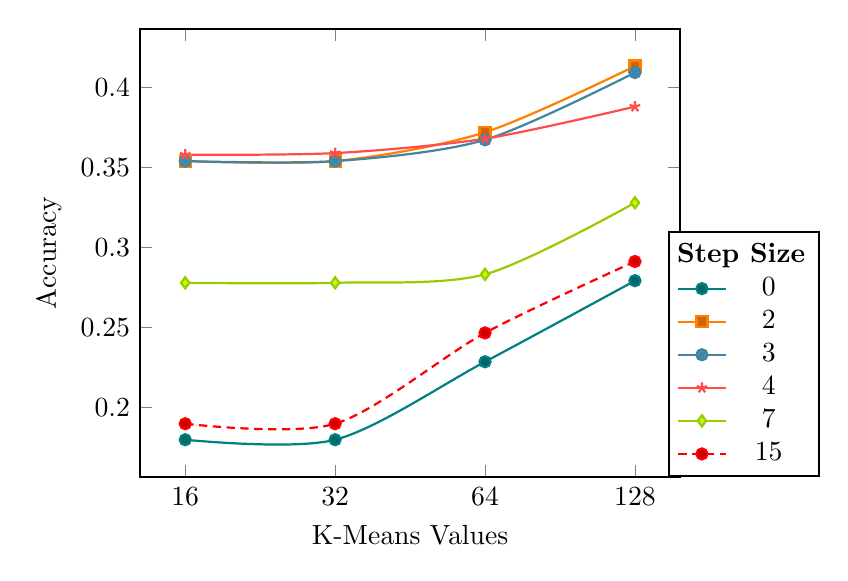
\begin{tikzpicture}
				    \begin{axis}
				        [
				        ,xlabel=K-Means Values
				        ,ylabel=Accuracy
				        ,yticklabel style={/pgf/number format/fixed}
				        ,xtick=data
				        ,xticklabels={16, 32, 64, 128}
				        ,legend style={at={(1.26 ,0.00)},anchor=south east}
				        ,cycle list name=exotic
				        ,smooth
				        ,thick
				        ,mark=*
				        ]
   						\addlegendimage{empty legend}
				        \addplot coordinates
				        {(0,0.18) (1,0.18) (2,0.2287) (3,0.2793)};
				        \addplot coordinates
				        {(0,0.354) (1,0.354) (2,0.372) (3,0.4133)};
				        \addplot coordinates
				        {(0,0.354) (1,0.354) (2,0.3673) (3,0.4093)};
				        \addplot coordinates
				        {(0,0.358) (1,0.359) (2,0.368) (3,0.388)};
				        \addplot coordinates
				        {(0,0.278) (1,0.278) (2,0.2833) (3,0.328)};
				        \addplot coordinates
				        {(0,0.19) (1,0.19) (2,0.2467) (3,0.2913)};
				        \addlegendentry{\hspace{-.7cm}\textbf{Step Size}};
   						\addlegendentry{0}
   						\addlegendentry{2}
   						\addlegendentry{3}
   						\addlegendentry{4}
   						\addlegendentry{7}
   						\addlegendentry{15}
				    \end{axis}
				\end{tikzpicture}
				\captionsetup{width=.9\textwidth}
				\captionof{figure}{Accuracy results with different k-nearest neighbor values and step sizes where k-means value is 128.}
			 \end{minipage}
			 \hfill
			\begin{minipage}{0.49\textwidth}
				\centering
				\begin{tabular}{ | c | c | c | }
				  	\hline			
				  	\bf step size & \bf k-NN & \bf accuracy \\
					\hline
				   	\multirow{4}{*}{0} & 1 & 0.18 \\
				   	\cline{2-3}
				   	& 2 & 0.18 \\
				   	\cline{2-3}
				   	& 4 & 0.2287 \\
				   	\cline{2-3}
				   	& 16 & 0.2793 \\
				  	\hline
				   	\multirow{2}{*}{2} & 1 & 0.354 \\
				   	\cline{2-3}
				   	& 2 & 0.354 \\
				   	\cline{2-3}
				   	& 4 & 0.372 \\
				   	\cline{2-3}
				   	& 16 & 0.4133 \\
				  	\hline
				   	\multirow{2}{*}{3} & 1 & 0.354 \\
				   	\cline{2-3}
				   	& 2 & 0.354 \\
				   	\cline{2-3}
				   	& 4 & 0.3673 \\
				   	\cline{2-3}
				   	& 16 & 0.4093 \\
				  	\hline
				   	\multirow{2}{*}{4} & 1 & 0.358 \\
				   	\cline{2-3}
				   	& 2 & 0.358 \\
				   	\cline{2-3}
				   	& 4 & 0.368 \\
				   	\cline{2-3}
				   	& 16 & 0.388 \\
				  	\hline
				   	\multirow{2}{*}{7} & 1 & 0.278 \\
				   	\cline{2-3}
				   	& 2 & 0.278 \\
				   	\cline{2-3}
				   	& 4 & 0.2833 \\
				   	\cline{2-3}
				   	& 16 & 0.328 \\
				  	\hline
				   	\multirow{2}{*}{15} & 1 & 0.19 \\
				   	\cline{2-3}
				   	& 2 & 0.19 \\
				   	\cline{2-3}
				   	& 4 & 0.2467 \\
				   	\cline{2-3}
				   	& 16 & 0.2913 \\
				  	\hline
				\end{tabular}
				\captionsetup{width=.8\textwidth}
				\captionof{table}{Accuracy results with different k-nearest neighbor values and step sizes where k-means value is 128.}
			\end{minipage}
		\end{minipage} \\
		
		As it can be seen above, accuracy is same with k-nearest neighbor values 1 and 2 due to my k-nearest neighbor implementation. As k-nearest neighbor value increases, the accuraccy is also increased. That is because validation or test image is checked with more data and it provides better result. 
        
        \item What is accuracy and how do you evaluate it? Briefly explain.
        
		Accuracy is the percentage of correct prediction count divided with total number of validation data. If a validation image is predicted the same as its groundtruth class then it is predicted correctly.
		k-Nearest Neighbor implementation: I have the train and validation data histograms (bag of features) and their class labels. For each validation BoF, I calculate its L2 distance to each train BoF and get the closest $k$ values. The predicted class is selected from the $k$ closest images.
		
        \item Give confusion matrices for classification results of several combinations of your choice. For example, you may try different $k$ values (of k-means and k-nearest neighbor, seperately, of course) or local features.

		I got results for combinations of k-Means 16, 32, 64, 128, step size 0, 2, 3, 4, 7, 15 and k-Nearest Neighbors 1, 2, 4, 16 configurations. The most accurate configuration's confusion matrices with different step sizes are below with their parameters:

        \begin{figure}[!h]
			\centering
			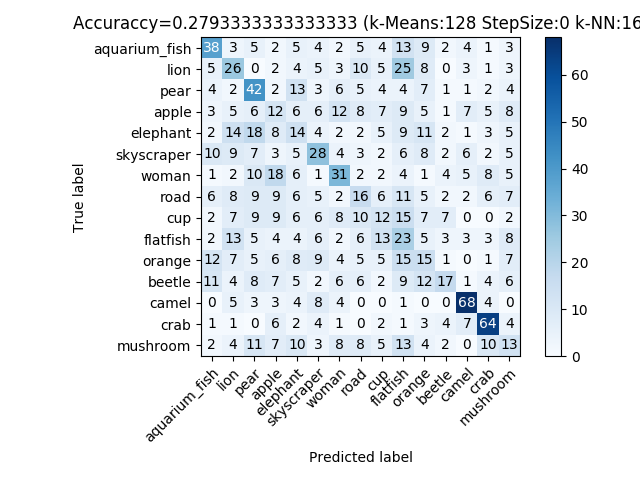
\includegraphics[width=0.48\textwidth]{Figure_1-0.png}
			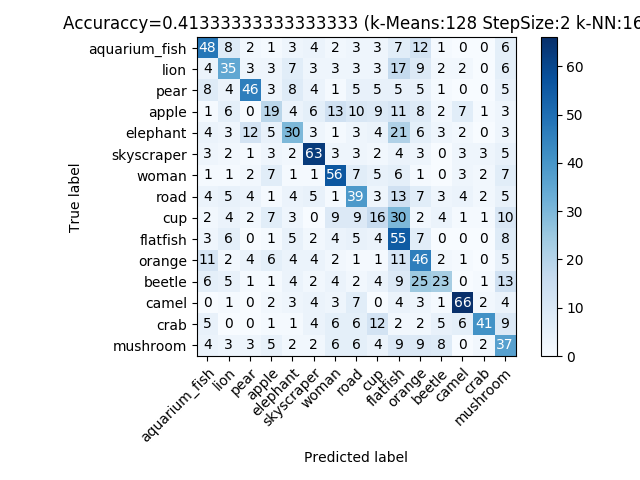
\includegraphics[width=0.48\textwidth]{Figure_1-1.png}
		\end{figure}
        \begin{figure}[!h]
			\centering
			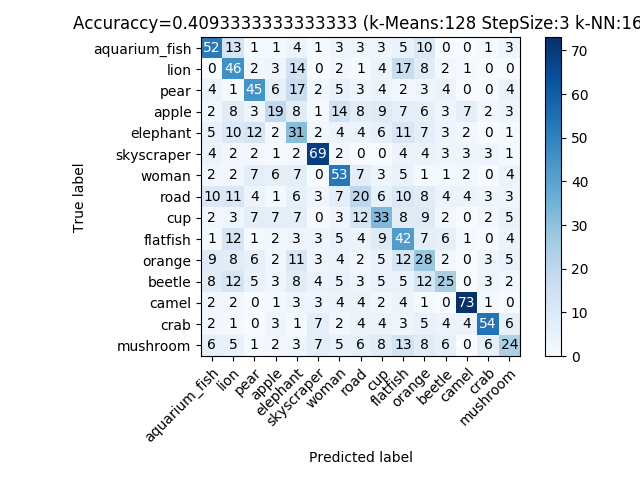
\includegraphics[width=0.48\textwidth]{Figure_1-2.png}
			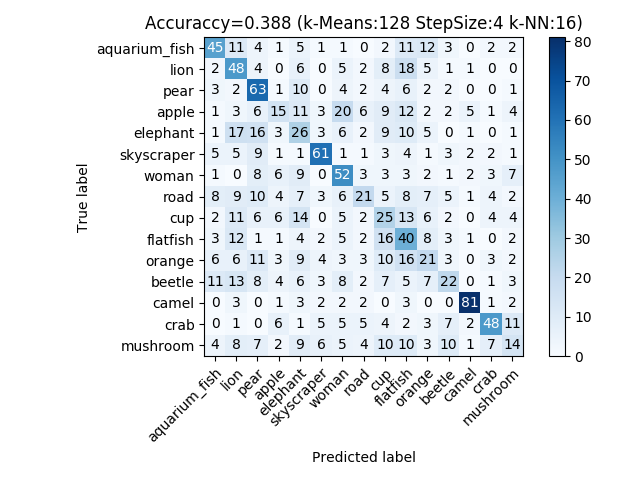
\includegraphics[width=0.48\textwidth]{Figure_1-3.png}
		\end{figure}
        \begin{figure}[!h]
			\centering
			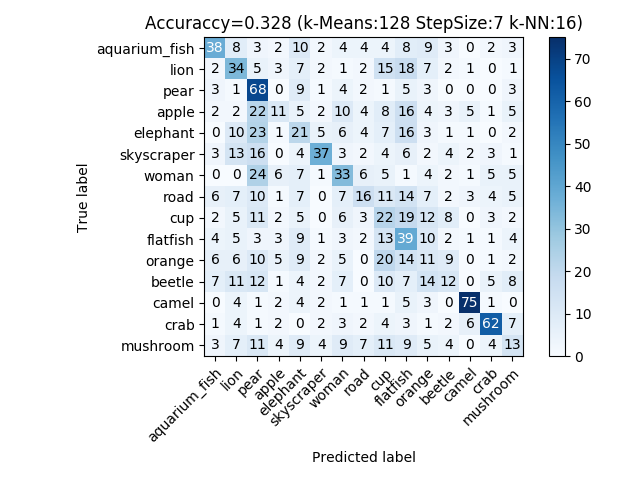
\includegraphics[width=0.48\textwidth]{Figure_1-4.png}
			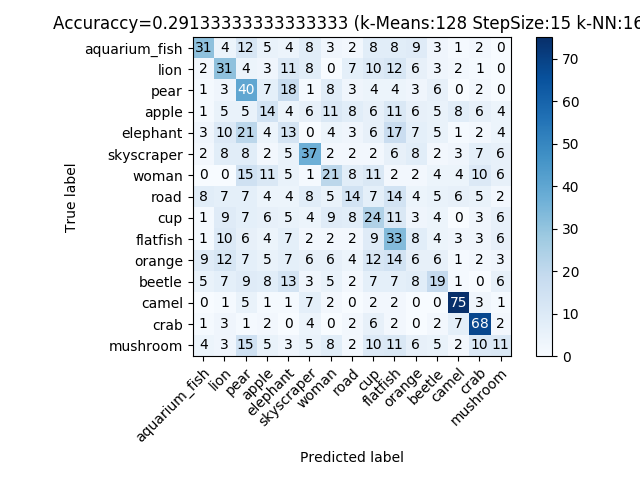
\includegraphics[width=0.48\textwidth]{Figure_1-5.png}
			\caption{Confusion matrices of best configurations for different step sizes.}
		\end{figure}
		
    \end{itemize}
\pagebreak
\section{Your Best Configuration (30 pts)}
    \begin{itemize}
        \item You may try different combinations by changing parameters above. Simply give your best accuracy for the validation set. How did you decide to use this configuration?
        
        My best accuracy for the given validation set is \textbf{k-Means 128}, \textbf{step size 2} and \textbf{k-Nearest Neighbor 16}. It achieves \textbf{0.4133} accuracy over the validation data. I decided the best configuration values by following the homework's report. The first, I discovered that Dense-SIFT is better than SIFT when step size is small. The second, I learnt that k-Means with large value such as 128 is better in accuracy than the smaller values. And the last, higher k-Nearest Neigbor value such as 16 performed well than the smaller values. Maybe, higher k-Means and k-Nearest Neighbor values or step size 1 achieve better results because I couldn't see where the decrease starts in the accuracy.
        
        \item Explain your setup for this best accuracy. How can we reproduce your result using your code?
        
        My best accurate configuration for the given validation set is \textbf{k-Means 128}, \textbf{step size 2} and \textbf{k-Nearest Neighbor 16}. It achieves \textbf{0.4133} accuracy over the validation data.
        
		For obtaining the validation data scores:        
        
		\begin{lstlisting}
		python3 k_means_clustering.py PATH_TO_DATASET K-MEANS STEP_SIZE
		python3 k_nearest_neighbors.py PATH_TO_DATASET K-MEANS STEP_SIZE KNN
		\end{lstlisting}
		
		For classifying the test data:
        
		\begin{lstlisting}
		python3 k_means_clustering.py PATH_TO_DATASET K-MEANS STEP_SIZE
		python3 classifier.py PATH_TO_DATASET PATH_TO_TEST_FOLDER K-MEANS STEP_SIZE KNN
		\end{lstlisting}
		
		\textbf{Note} that running the program might take time. It caches the important data for later uses. The given dataset's file structure is important for my code to run!
        
        \item Visualize confusion matrix for your best classification and briefly interpret the values.
        
        \begin{figure}[!h]
			\centering
			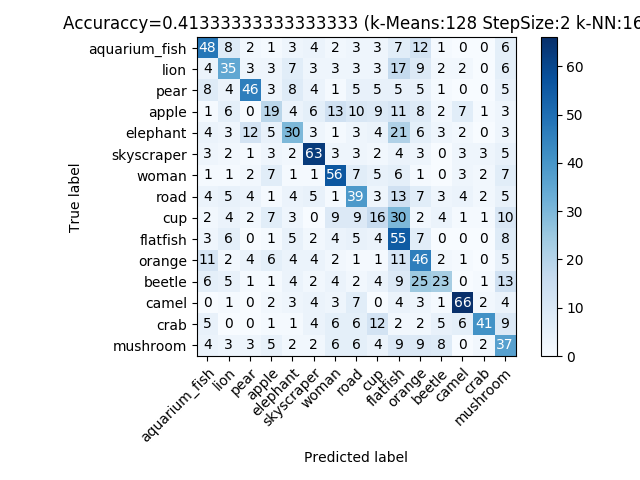
\includegraphics[width=1\textwidth]{Figure_1-1.png}
			\caption{Confusion matrix of my best classification result in validation dataset.}
		\end{figure}
		
		The matrix is not normalized, but there are 100 images belong to each classes. If the classifier were the best, the each diagonal element would be 100 (and its color would be darker). However, it is not the case. \textbf{Camel} class has the best classification rate with $0.66$ and \textbf{cup} class has the lowest classification rate with $0.16$. If we sum the values on the diagonal and divided it with the total number of images, we get accuracy which is $620/1500=0.413$. We can learn which classes will be poorly classified from this matrix and we can reinforce those classes data in order to improve the classification accuracy.
    \end{itemize}

\section{Additional Comments and References}
	I used these links while doing the homework:
	
	\begin{itemize}
		\item\url{https://opencv-python-tutroals.readthedocs.io/en/latest/py_tutorials/py_feature2d/py_sift_intro/py_sift_intro.html}
		\item\url{https://stackoverflow.com/questions/33120951/compute-dense-sift-features-in-opencv-3-0/33702400}
		\item\url{https://scikit-learn.org/stable/modules/generated/sklearn.cluster.KMeans.html}
		\item\url{https://scikit-learn.org/stable/auto_examples/model_selection/plot_confusion_matrix.html#sphx-glr-auto-examples-model-selection-plot-confusion-matrix-py}
	\end{itemize}

\end{document}

